\section{Latch Etapa de memoria de datos - Etapa de escritura}
Contiene las senales que proviene desde la etapa de decodificaci\'on y adem\'as el dato que sale de la memoria de datos.

\begin{figure}[H]
\centering
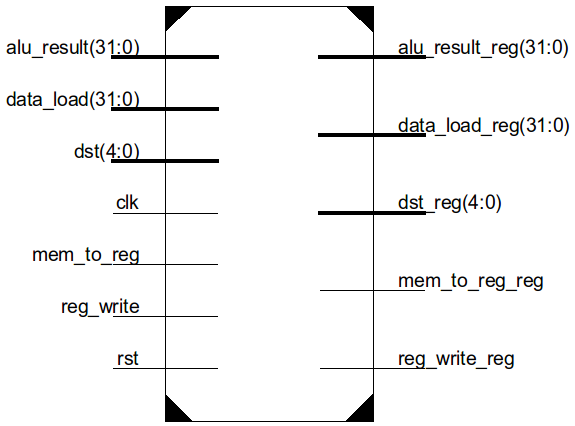
\includegraphics[scale=0.5]{img/latch_m_wb}
\caption{Latch Etapa de memoria - Etapa de Escritura}
\label{fig:latch_m_wb}
\end{figure}

Tiene como entradas:
\begin{itemize}
  \item \textbf{alu\_result}: Bus de 31 bits que toma el resultado que proviene de la operacion de la alu de la etapa de ejecucion.
  \item \textbf{data\_load}: Bus de 31 bits que contiene el dato que fue suministrado por la etapa de lectura de la memoria.
  \item \textbf{dst}: Bus de 5 bits que es el puntero al registro que se va a escribir en el banco de registros de la etapa de decodificaci\'on.
  \item \textbf{clk}: Reloj general del sistema.
  \item \textbf{mem\_to\_reg}: Senal que habilita la escritura del registro a la memoria.
  \item \textbf{reg\_write}: Senal que habilita la escritura de registros de la etapa de decodifici\'on.
  \item \textbf{rst}: Reset que vuelve al estado inicial de los registros. 
\end{itemize} 